\section{Laboratory work implementation}

\subsection{Tasks and Points}
\begin{enumerate}
	\item  Realizarea unei  aplicații mobile (Game)
	
\end{enumerate}

\subsection{Analiza lucrarii de laborator}

Click on \href{https://github.com/OctavianCoroletchiTI154/MIDPS.git}{"Link"} or copy \url{https://github.com/OctavianCoroletchiTI154/MIDPS.git} pentru repozitoriul meu.
\par Task a: \\
Am realizat un simplu joc ce dateaza din 1984, Tetris. Este un simplu joc in care interactionam cu anumite forme, pentru a forma o linie orizontala fara spatii si a eliminao. Astfel obtinem 10 puncte. Acesta este intreg principiu al jocului. \\
Eu am realizat jocul in xCode, valabil pentru Apple's Environment. Acesta a fost executat in limbajul Swift creat de in special pentru dezvoltarea produselor pe platforma iOS, MacOS, watchOS si tvOS. Acesta este un limbaj modern, care are un potential uimitor in viitor. Contine multiple utilitati care face munca dezvoltatorului mai usoara. Are o sintaxa mai speciala fata de celelalte, cum ar fi C, C++ si Java. Pentru inceput a fost greu pentru a te obisnui cu unele scrieri.\\
Jocul va folosi SpriteKit. Acesta este un set de APIs oferite de iOS SDK(software development kit) care ofera suport pentur dezvoltarea jocurilor 2D. Deaceea nu va fi nevoie de alte utilitati. 
Intreg joc se bazeaza pe un array de 10 coloane si 20 rinduri. Aici implementam toate necesare pentru jocul nostru. Pentru a interactiona cu un tablou bidimensional, am creat o clasa speciala Array2D pentru a putea face acest lucru posibil, deoarece Swift foloseste un index pentru numerotarea oricarui loc in array. \\
Clasa Block va crea formele noastre pentru fiecare obiect in parte.  Acesta va folosi clasa Shape care va defini bucatile Tetromino. Aici vom implementa rotirile la fiecare actiune, la 90 grade. Clasa Shape, va folosi subclase precum SquareShape, TShape, LineShape, LShape, JShape, SShape, ZShape. Toate aceste subclase vor forma toate formele din Tetromino. In clasa Tetris, se vor specifica toate regulile jocului. La final am adaugat toate actiunile care le va face utilizatorul, atunci cind va atinge display-ul, va misca cu degetul in stinga sau dreapta, sau va pune figura jos cu o  miscare in jos. 
In Fig a-1, se poate observa rezultatul final al jocului.
\clearpage


\subsection{Imagini}
\begin{center}
\vspace{30 mm}
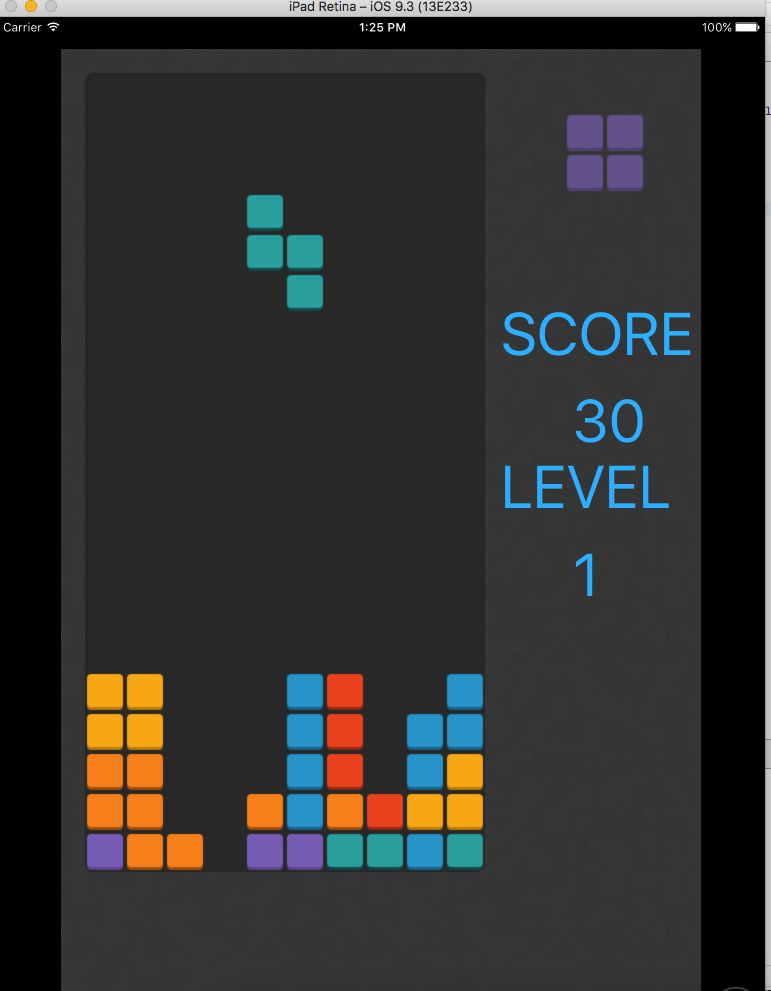
\includegraphics[scale=0.37]{Test1} \\ 
Fig a-1 - "Rezultatul final al jocului" \\
\vspace{10 mm}




\end{center}


